% =====================================================================
%  Capítulo 7 — Tipos de agresores
% =====================================================================
\chapter{Tipos de agresores}

A continuación presentamos los tipos más comunes de agresores, según sus objetivos y su forma de proceder habitual, para desarrollar una estrategia personal según el caso. Debemos tener en cuenta que pueden presentar trastornos psiquiátricos o estar bajo la influencia de drogas: hay que determinar rápidamente si su condición es de inferioridad física (p.\,ej., alcohol) o lo contrario (p.\,ej., estimulantes), para actuar en consecuencia.

\begin{table}[h]
\centering
\renewcommand{\arraystretch}{1.3}
\small
\begin{tabularx}{\linewidth}{@{}>{\bfseries}l X l l@{}}
\toprule
\textbf{Objetivo} & \textbf{Táctica / Estrategia} & \textbf{Víctimas} & \textbf{Nombre} \\
\midrule
Dinero & Robo, atraco, tirón, secuestro\ldots{} & Hombres y mujeres & Ladrón \\
Ego & Peleas (normalmente sin estrategia, sucediéndose las técnicas) & Más hombres & Buscapeleas \\
Sexo / poder & Abordar por sorpresa o, mucho más a menudo, abusar de una relación de confianza previa & Más mujeres & Agresor sexual \\
Control & Violencia física y psicológica continuada dentro de la pareja o expareja & Mujeres & Maltratador \\
\bottomrule
\end{tabularx}
\end{table}

\section{Ladrón}

El delito más común es el robo con intimidación por armas o por número de delincuentes. Lo primero es establecer cuántos son, ya que podemos ser sorprendidas por cómplices en el momento de realizar una acción defensiva.

Enfrentarse a más de una persona no es aconsejable: se recomienda mantener la calma, entregar los bienes solicitados, no mirar fijamente los rostros (miradas fugaces; los delincuentes temen el reconocimiento) y no provocarles. Es decir, concluir la situación lo antes posible y resultar ilesa, dirigiéndose de inmediato a efectuar la denuncia aportando todos los datos posibles. Ningún objeto vale más que tu integridad.

\section{Buscapeleas}

Ser elegida por este tipo de individuo es un gran problema: generalmente no persigue el robo, sino que se trata de personas guiadas por el deseo de hacer daño (por satisfacción personal, por el público\ldots{}). Están acostumbrados a soportar dolor, tienen un gran repertorio de técnicas sucias y son poco proclives a abandonar mediante el diálogo. Suelen iniciar el ataque con un golpe de improviso.

\begin{itemize}
  \item En estos enfrentamientos no hay reglas: todo vale a efectos de ataque y defensa (como los golpes a genitales), y no se debe mostrar clemencia, porque el atacante no la tendrá.
  \item Busca elementos del entorno (palos, botellas\ldots{}) a modo de arma defensiva, valorando que exhibirlos puede escalar el conflicto si él también tiene acceso a armas o acompañantes. Se pueden usar paredes cercanas o el suelo para empujar contra ellos al rival.
  \item Pon al oponente en el peor terreno: llévalo hacia suelo desfavorable, colócate a un nivel más alto y, de noche, de espaldas a la luz (que le dé en la cara).
  \item Mantén la tranquilidad para no atacar a lo loco, sino a los puntos vulnerables que queden expuestos y con tus técnicas preferidas.
  \item No dudes: provoca una distracción verbal o arrojando algo a la cara, y de inmediato golpea con decisión, combinando manos y pies con técnicas sencillas.
  \item No te confíes: ni de las palabras ni de una aparente rendición; no des nunca la espalda ni relajes la atención.
  \item Termina lo más rápido posible y retírate del lugar de inmediato.
\end{itemize}

Estadísticamente, según el género del agresor su forma de actuar es distinta. Si es hombre, lo habitual son golpes a puño cerrado, golpes ascendentes si la agredida se inclina, abrazos al cuerpo y cuello, patadas frontales a genitales o circulares al pecho y cabeza, y cabezazos en la corta distancia. Si es mujer, lo habitual son golpes a mano abierta y arañazos, estirones al suelo, agarres al pelo, cuerpo y cuello, pisotones y patadas descendentes, y escupitajos en la corta distancia.

\newpage

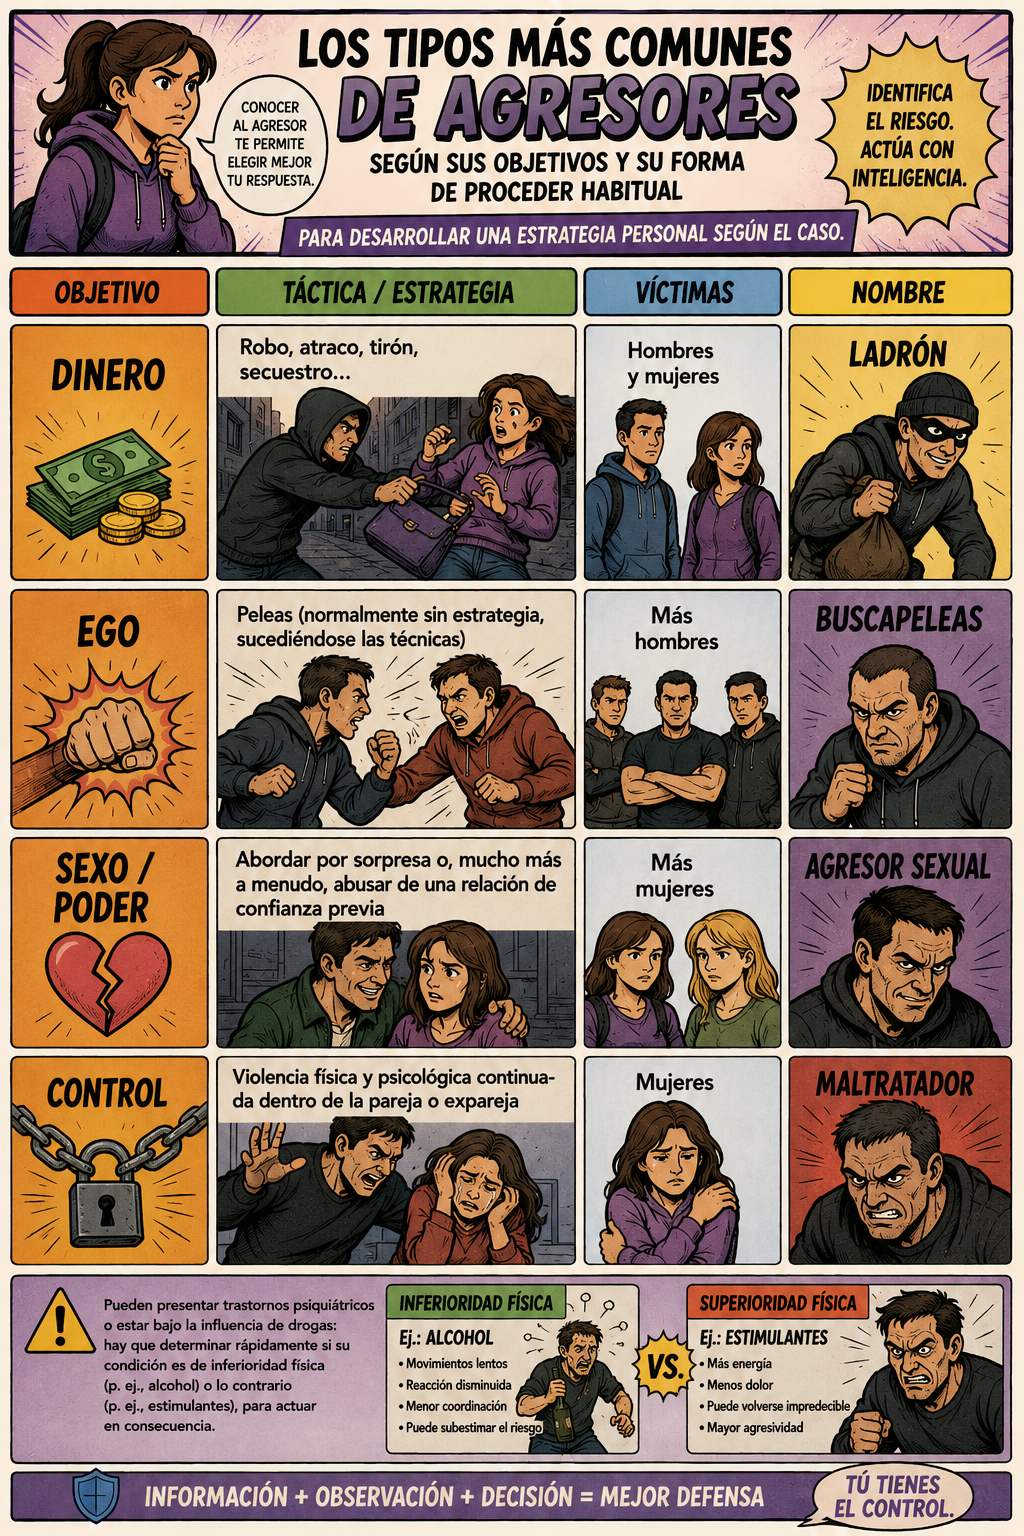
\includegraphics[width=\linewidth]{figures/agresores.png}